% !TEX TS-program = pdflatex
% !TEX encoding = UTF-8 Unicode

% This is a simple template for a LaTeX document using the "article" class.
% See "book", "report", "letter" for other types of document.

\documentclass[11pt]{article} % use larger type; default would be 10pt

\usepackage[utf8]{inputenc} % set input encoding (not needed with XeLaTeX)

%%% Examples of Article customizations
% These packages are optional, depending whether you want the features they provide.
% See the LaTeX Companion or other references for full information.

%%% PAGE DIMENSIONS
\usepackage{geometry} % to change the page dimensions
\geometry{letterpaper} % or letterpaper (US) or a5paper or....
% \geometry{margin=2in} % for example, change the margins to 2 inches all round
% \geometry{landscape} % set up the page for landscape
%   read geometry.pdf for detailed page layout information

\usepackage{graphicx} % support the \includegraphics command and options
\graphicspath{{fig/}}

%%% PACKAGES
\usepackage{booktabs} % for much better looking tables
\usepackage{array} % for better arrays (eg matrices) in maths
\usepackage{paralist} % very flexible & customisable lists (eg. enumerate/itemize, etc.)
\usepackage{verbatim} % adds environment for commenting out blocks of text & for better verbatim
\usepackage{subfig} % make it possible to include more than one captioned figure/table in a single float
\usepackage{gensymb} % general symbols
\usepackage{amsmath} % math symbols
\usepackage{amsfonts} % for symbols
\usepackage{amssymb} % for symbols
\usepackage{placeins}% to prevent floating between sections
\usepackage{subfig} % for subfloats
\usepackage{epstopdf} % for including EPS files
\usepackage{lpic}



% These packages are all incorporated in the memoir class to one degree or another...

%%% HEADERS & FOOTERS
\usepackage{fancyhdr} % This should be set AFTER setting up the page geometry
\pagestyle{fancy} % options: empty , plain , fancy
\renewcommand{\headrulewidth}{0pt} % customise the layout...
\lhead{}\chead{}\rhead{}
\lfoot{}\cfoot{\thepage}\rfoot{}

%%% SECTION TITLE APPEARANCE
\usepackage{sectsty}
\allsectionsfont{\sffamily\mdseries\upshape} % (See the fntguide.pdf for font help)
\setcounter{secnumdepth}{-1}
% (This matches ConTeXt defaults)

%%% ToC (table of contents) APPEARANCE
\usepackage[nottoc,notlof,notlot]{tocbibind} % Put the bibliography in the ToC
\usepackage[titles,subfigure]{tocloft} % Alter the style of the Table of Contents
\renewcommand{\cftsecfont}{\rmfamily\mdseries\upshape}
\renewcommand{\cftsecpagefont}{\rmfamily\mdseries\upshape} % No bold!

%%% Custom Commands and Parameters
\providecommand{\e}[1]{\ensuremath{\times 10^{#1}}}
\newcolumntype{C}[1]{>{\centering\let\newline\\\arraybackslash\hspace{0pt}}m{#1}}

%%% END Article customizations

%%% The "real" document content comes below...

\title{Analog Electronics Final Project Report}
\author{Ankur Dhar and James Ryan Schloss}
\date{\today} % Activate to display a given date or no date (if empty),
         % otherwise the current date is printed 

\begin{document}
\maketitle
\section{Overview}
The goal of this project is to create an analog circuit that can process the output of an accelerometer, interpret the orientation, and based on set values produce the required output to drive four motors on a quadcopter to balance the system.

\section{Control Circuit}
For this project we chose an accelerometer from Freescale Semi (FXLN8361QR1) which operated between 1.7\,V and 3.6\,V. The device can also toggle between a low sensitivity mode ($\pm8g$) and a high sensitivity mode ($\pm2g$). When the power is supplied and mode set, the accelerometer outputs three voltages proportional to the acceleration in X, Y, and Z.\\
Thus on level ground at rest, the accelerometer should measure a net acceleration of $[0,0,-g]$. However, at zero acceleration, the device outputs an offset voltage of 0.75\,V, thus the equilibrium position in terms of voltage will be $[0.75\,V,0.75\,V,0.979\,V]$.\\
To determine this equilibrium, we need to integrate the Z signal twice to determine the net displacement, and select for the height we wish to hover at with a comparator. Then to balance, we also integrate both X and Y signals once to select for zero velocity. Since the comparator will output a rail voltage based on the net difference between measured value and set point, it must be scaled to appropriately control the motors to restore balance.

\section{Motor Control}
To control the motors, it is first important to understand the motors themselves. Quadcopters no longer use simple DC motors to control their speed, since they are not precise enough. Instead, they use what is known as three-phase AC signals. Each AC signal is $120\deg$ out of phase with each other, to trigger one of three electromagnet in the motor.\\
The frequency determines the rpm, which is precisely controlled by an electronic speed controller (ESC). This ESC measures the back emf of the first two poles to determine the phase shift of the third pulse.\\
The ESC in turn is controlled by a pulse width modulated (PWM) square wave from a central control system, such as a micro-controller or an analog circuit. The throttle it applies to the motors is controlled by the duty cycle of the wave, which can be simply generated by using a triangle wave and a comparator.\\
By comparing the output of the triangle wave to a set voltage, the resultant signal will either go to zero or the upper rail, with the width of the pulse equaling the width of the triangle wave that is above the set voltage. This the duty cycle of the square wave can be controlled simply by adjusting the set voltage of the comparator.\\
Figure~\ref{fig:PWM} shows the required circuit to accurately create the PWM signal. Testing this circuit revealed that a set voltage range 2 and 4V results in a duty cycle between 25\% to 65\%. The triangle wave itself needs to range from 0 to 5V to register properly.
\begin{figure}[h]
	\centering
	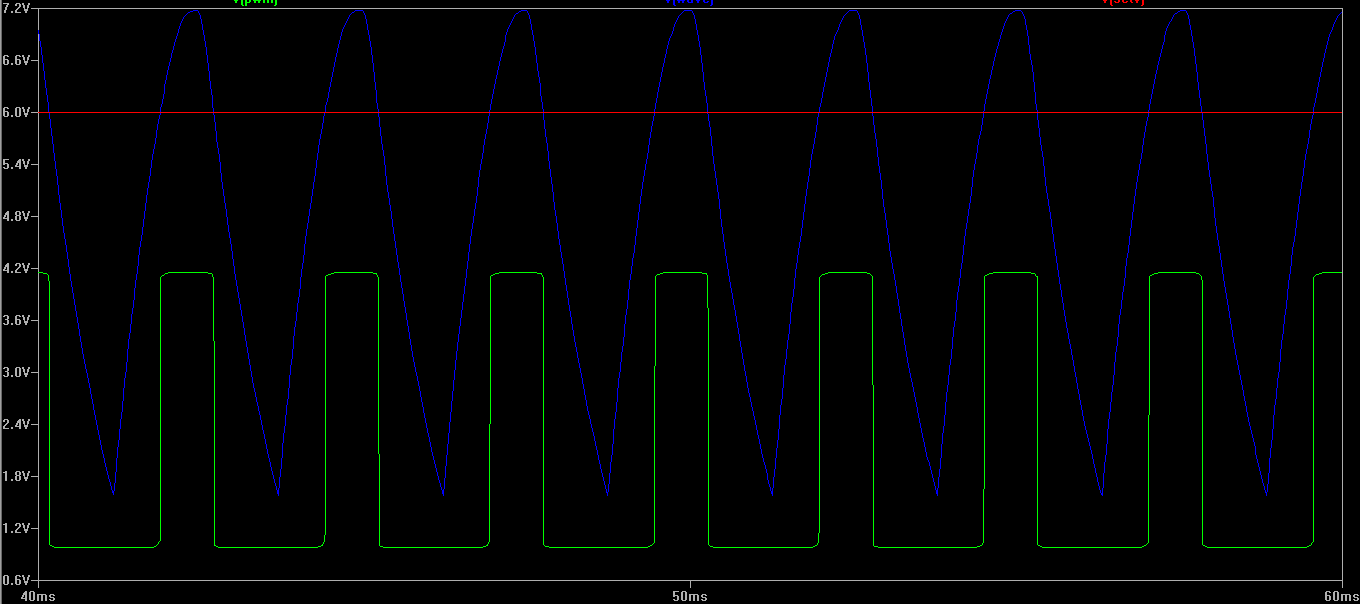
\includegraphics[width=\textwidth]{PWM}
	\caption{Schematic of PWM Circuit, consisting of a triangle wave, a set voltage, an opamp acting as a comparator, and a low pass filter.}
	\label{fig:PWM}
\end{figure}
\section{Mechanical Design}
The quadcopter itself had very few mechanical constraints, however the chassis did need to accommodate the following parts at minimum:
\begin{itemize}
\item Motors (x4)
\item ESC (x4)
\item Battery
\item Central control board
\item TTL board (x4)
\end{itemize}
The only parts that have an exact mechanical requirement are the motors, which have threaded holes for M3 bolts at the bottom to panel mounting. Thus it was decided to utilize the 3D printer at OIST to produce a custom designed chassis for the quadcopter, as shown in Figure~\ref{fig:chassis}.
\begin{figure}[h]
	\subfloat[3D Render in Solidworks]{
	\centering
	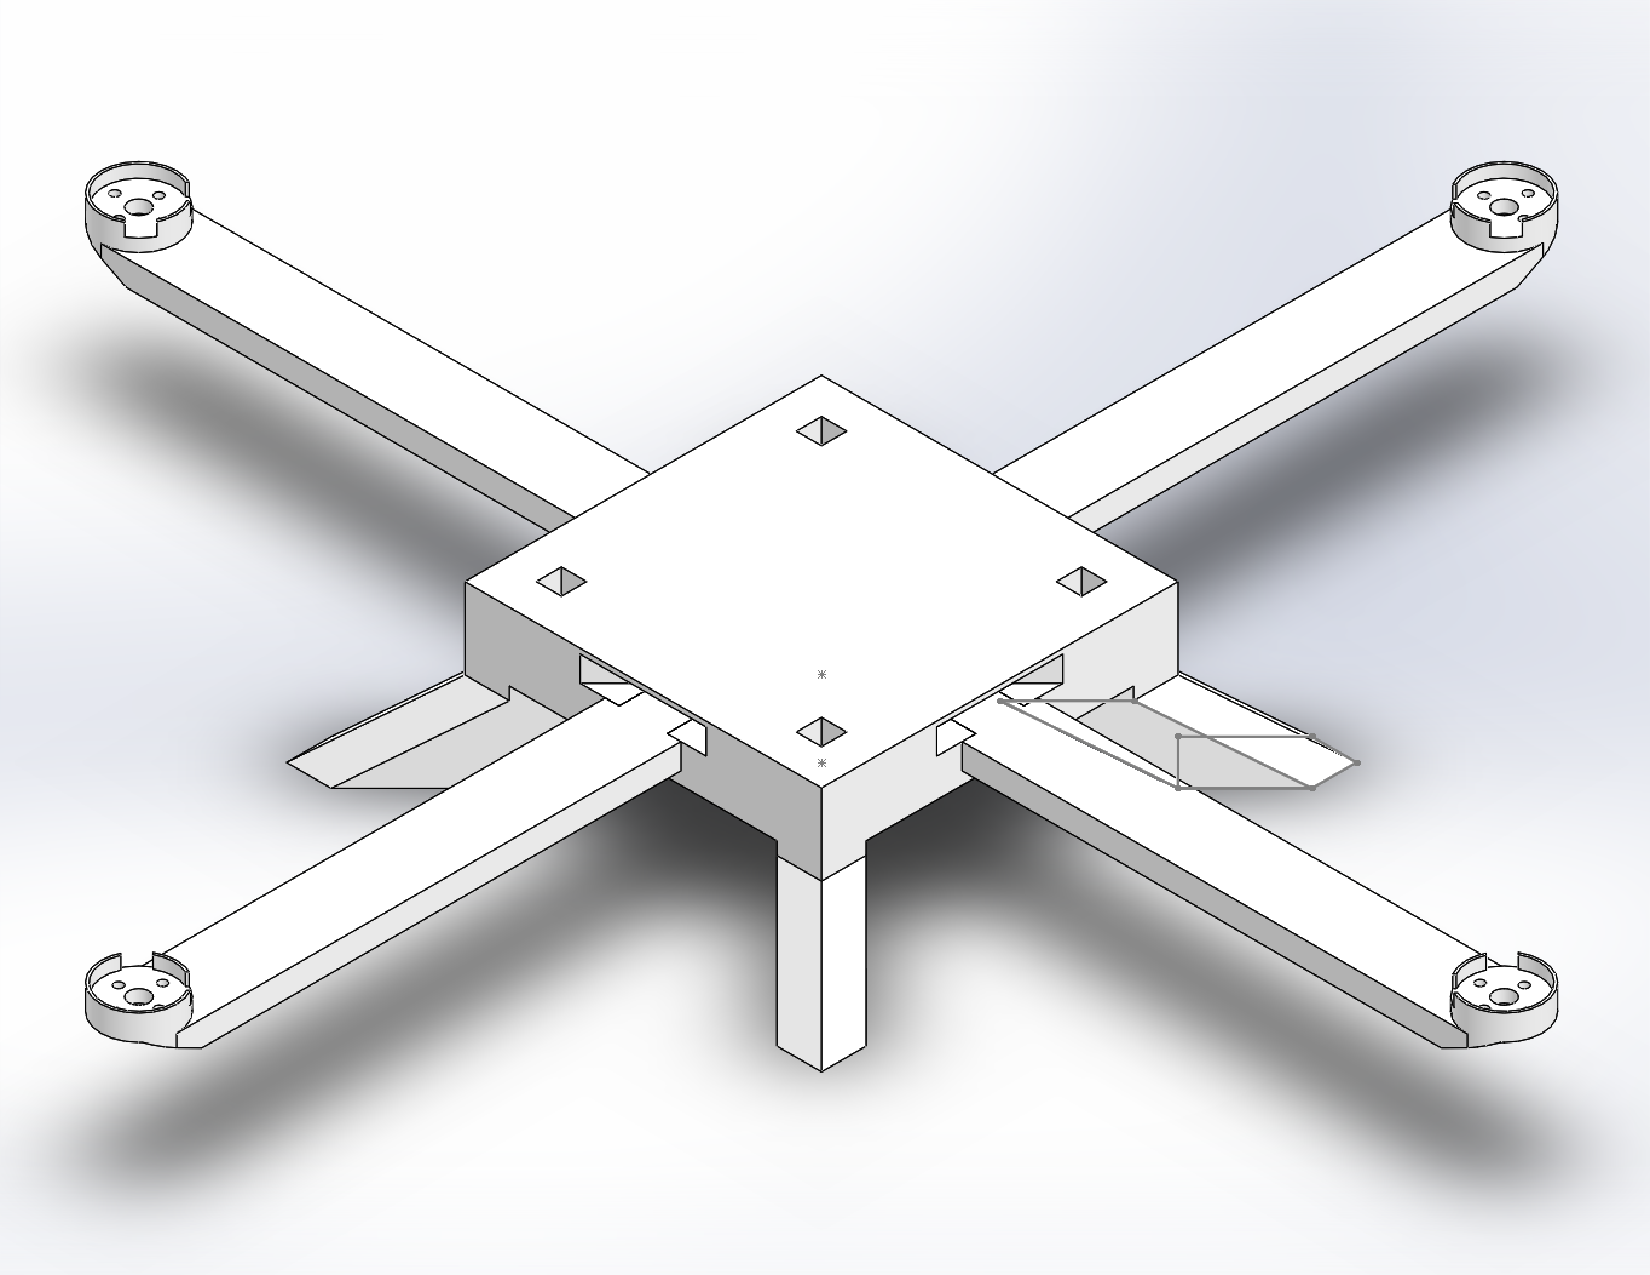
\includegraphics[width=.5\textwidth]{Quadcopter2D}
	}
	\subfloat[3D Printed Chassis with motors attached.]{
	\centering
	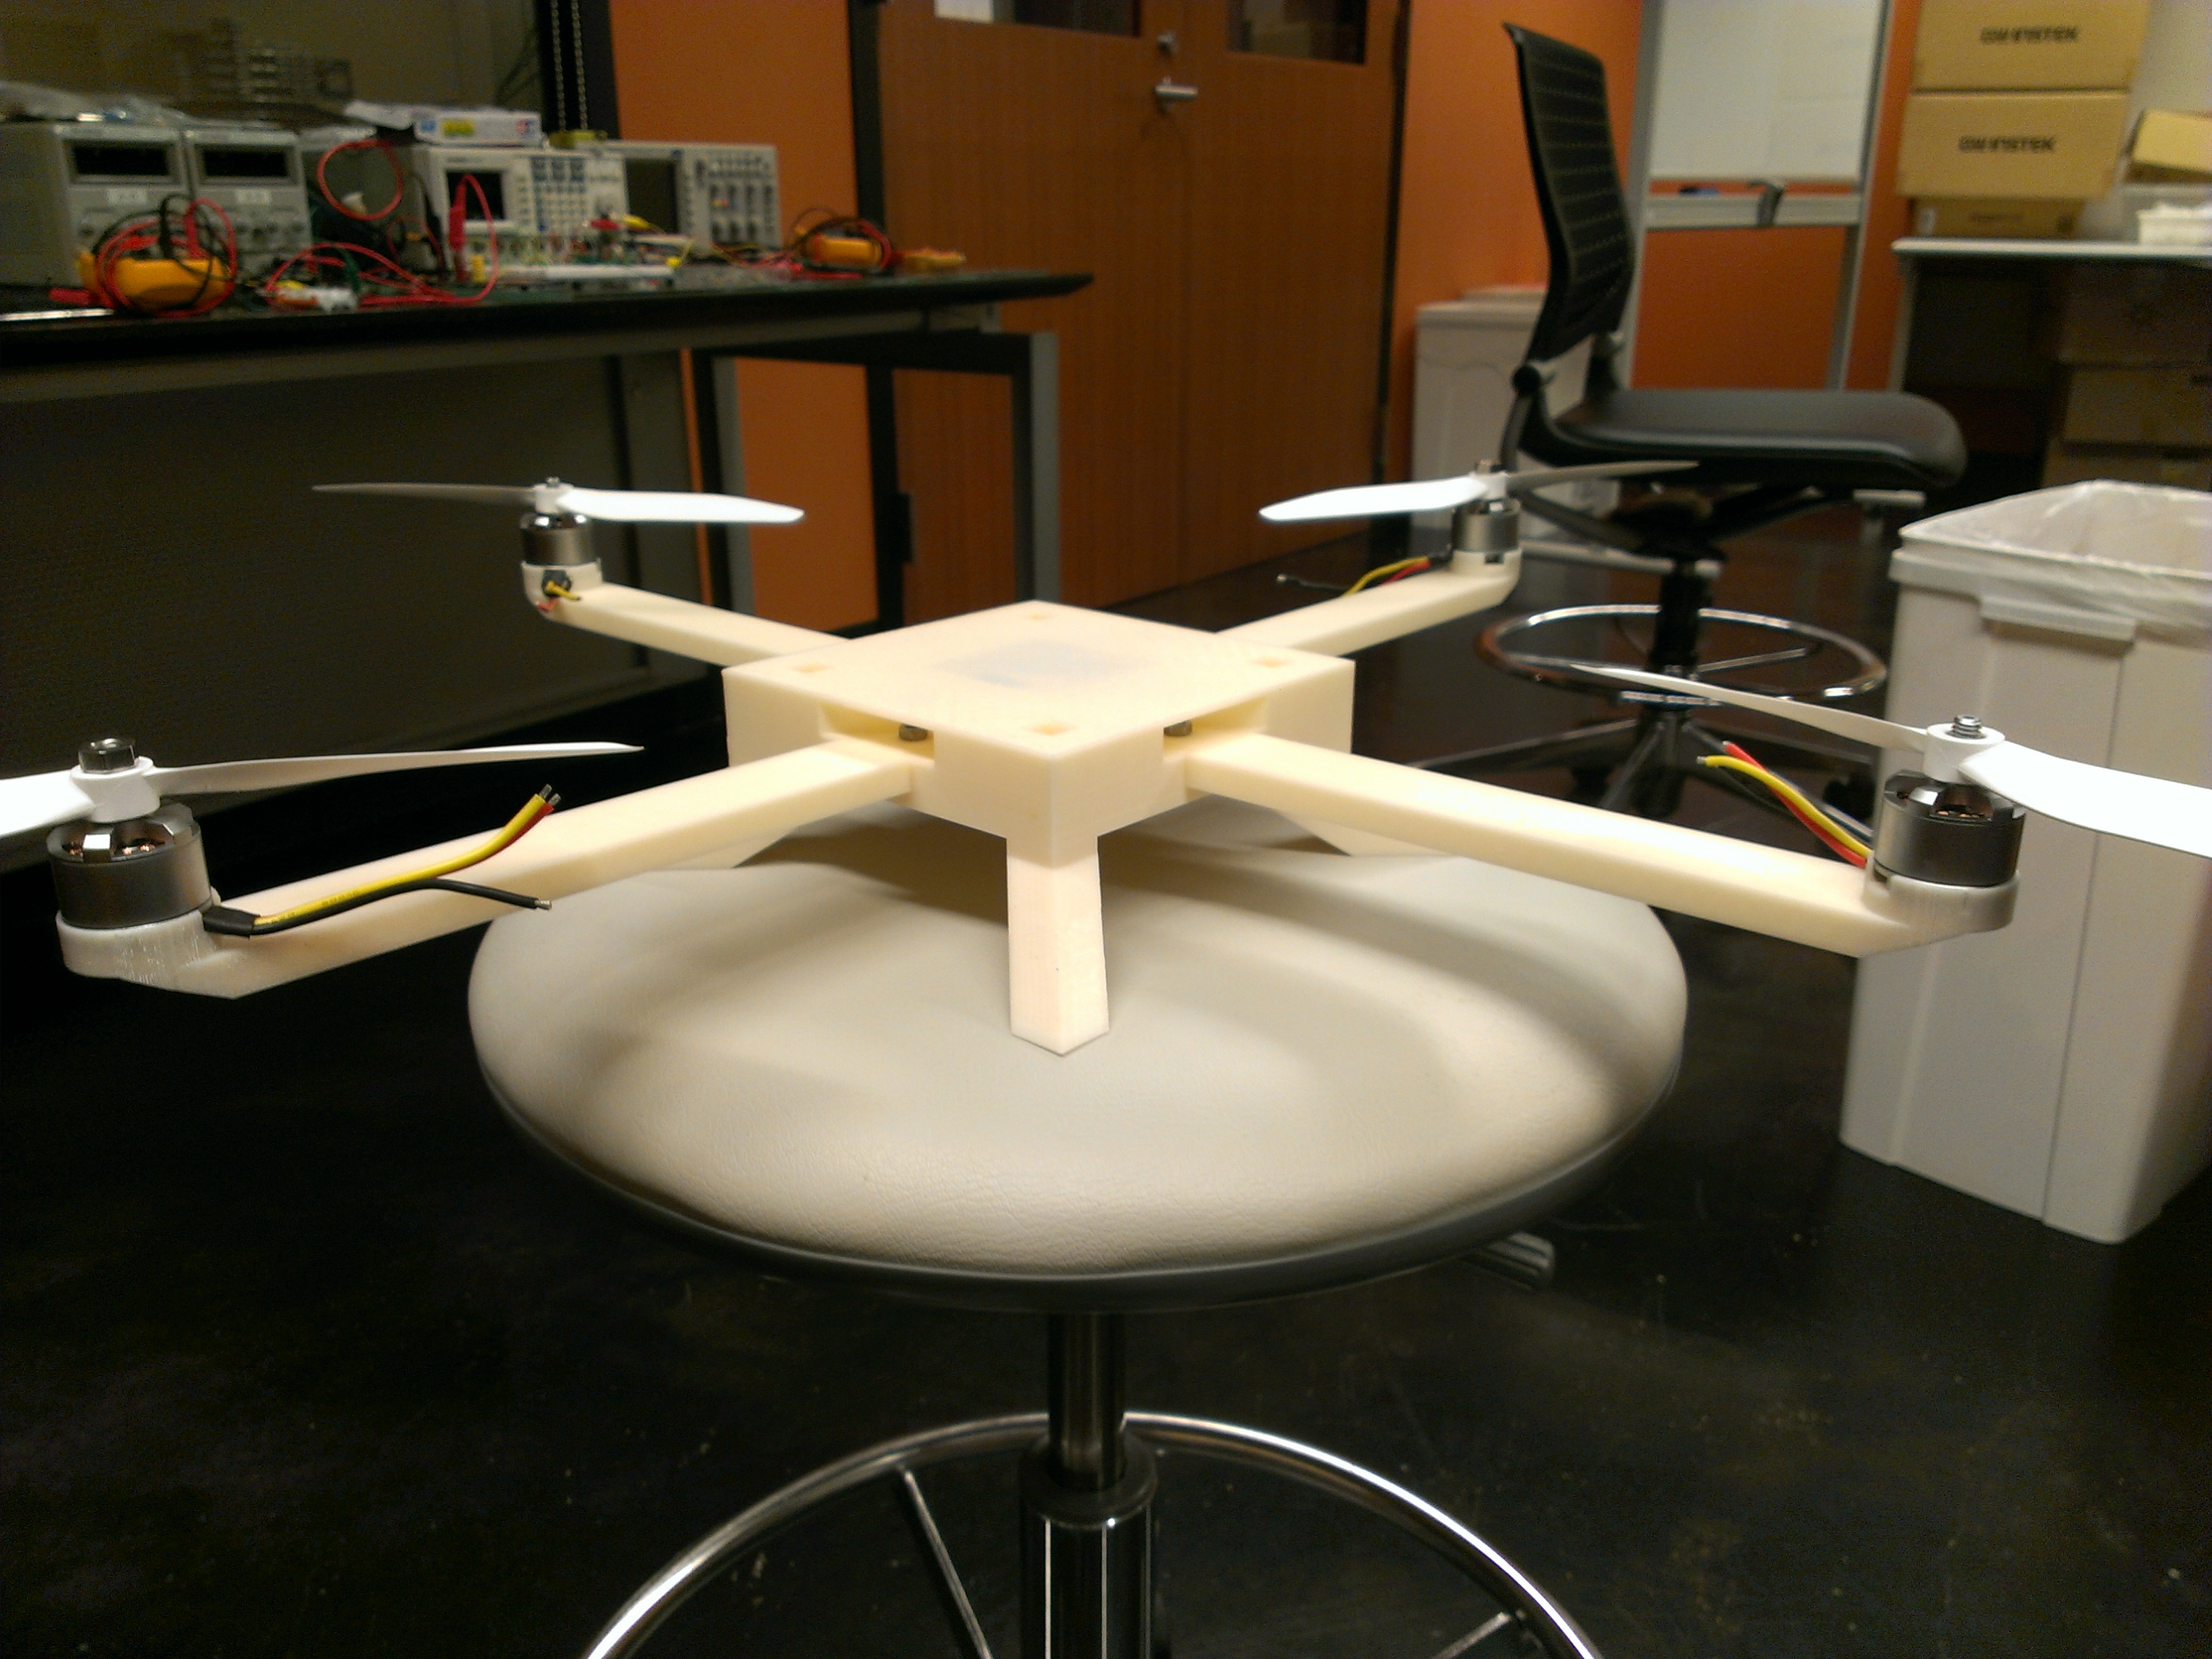
\includegraphics[width=.5\textwidth,clip=true,trim= 0 50 200 0]{Chassis}	
	}
	\caption{3D render of quadcopter chassis, with room for motors, battery, and requisite electronics.}
	\label{fig:chassis}
\end{figure}
Each arm has room for the motor to be mounted, along with space for the corresponding ESC to be mounted underneath with zip ties. Each arm locks into the central body, and is secured using an M5 bolt. The top section has holes to allow zip ties to wrap around the inner section to hold down the central electronics. Finally the bottom of the central piece has an additional hollowed section to more zip ties to hold the battery underneath, keeping the center of gravity low.
\section{Feedback}
The feedback mechanism in this system is not strictly electrical, but related through the orientation of the copter. The motors represent the final output stage of the control circuit, which will affect the orientation of the quadcopter. This in turn affects the output voltages of the accelerometer, which represent the inputs of the control circuit.\\
Thus to properly describe the feedback of this circuit, it is important to understand how much thrust the motors supply, and how that force twists the orientation of the quadcopter. In order to do this, the thrust must be characterized as a function of voltage, which is described in the appendix of this report.

\section{Problems and Issues}
This project ran into a lot of setbacks, mostly logistical but also due to poor planning. The initial concept of this project assumed that the quadcopter motors we would buy were simply DC motors, as opposed to three-phase AC motors. DC motors would have required a much simpler design, and proven more feasible for a project of this scope. Instead we were forced to redo our entire design to account for our quadcopter motors.\\
After some experimentation in building a three-phase AC circuit and consultation with online forums, we realized not only would this not be enough, but that we could not power the motors without a minimum of 8\,A, well beyond the capabilities of the power supplies provided. This required us to put in a second order for an appropriate battery and set of motor controllers.\\
Although we were able to finally obtain a functional accelerometer board to test, without the motors running there would be no need for a quadcopter. Thus while this report covers the entire scope of the intended project, the actual work achieved is limited to the control circuit and mechanical design.
\section{Conclusion}
In conclusion...
\newpage
\appendix
\section{Appendix A: Characterizing Motors}
Given a fixed motor and propeller combination, the only variable that can be adjusted in the RPM, which in turn determines the upward force each motor can generate. Although it would be possible to calculate this force numerically with the specific shape of the propeller, it is far more efficient to simply characterize the force as a function of voltage directly.\\

\end{document}
